\section{Results}

% ------------------------------------------------------------------------------
\begin{frame}
\frametitle{Agenda}
\tableofcontents[currentsection]
\end{frame}
% ------------------------------------------------------------------------------


% ------------------------------------------------------------------------------
\begin{frame}
\frametitle{Results: experiment 1}
\LARGE Any expectations?
\end{frame}
% ------------------------------------------------------------------------------

% ------------------------------------------------------------------------------
\begin{frame}
\frametitle{Results: experiment 1}
\begin{figure}

	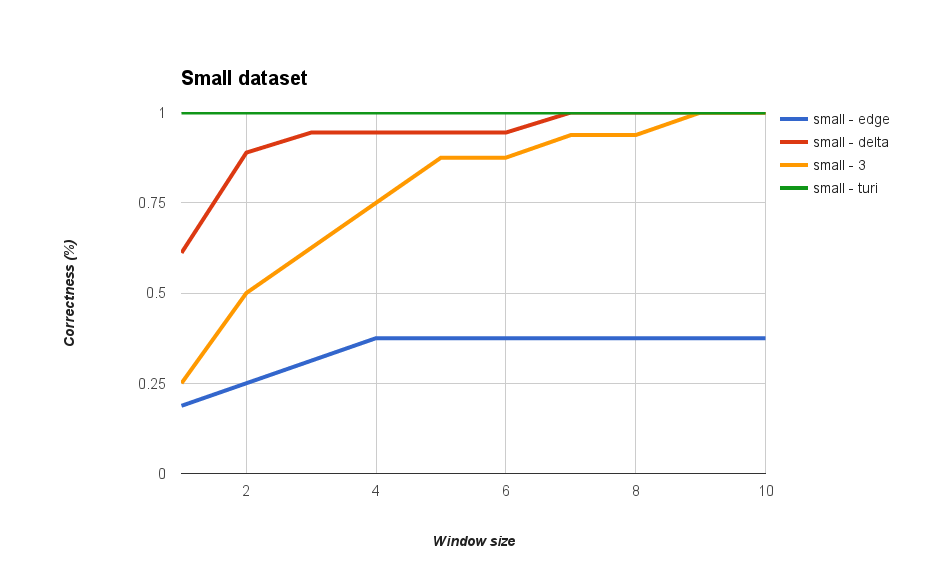
\includegraphics[width=\textwidth]{small.png}

\end{figure}
\end{frame}
% ------------------------------------------------------------------------------

% ------------------------------------------------------------------------------
\begin{frame}
\frametitle{Results: experiment 1}
\begin{figure}

	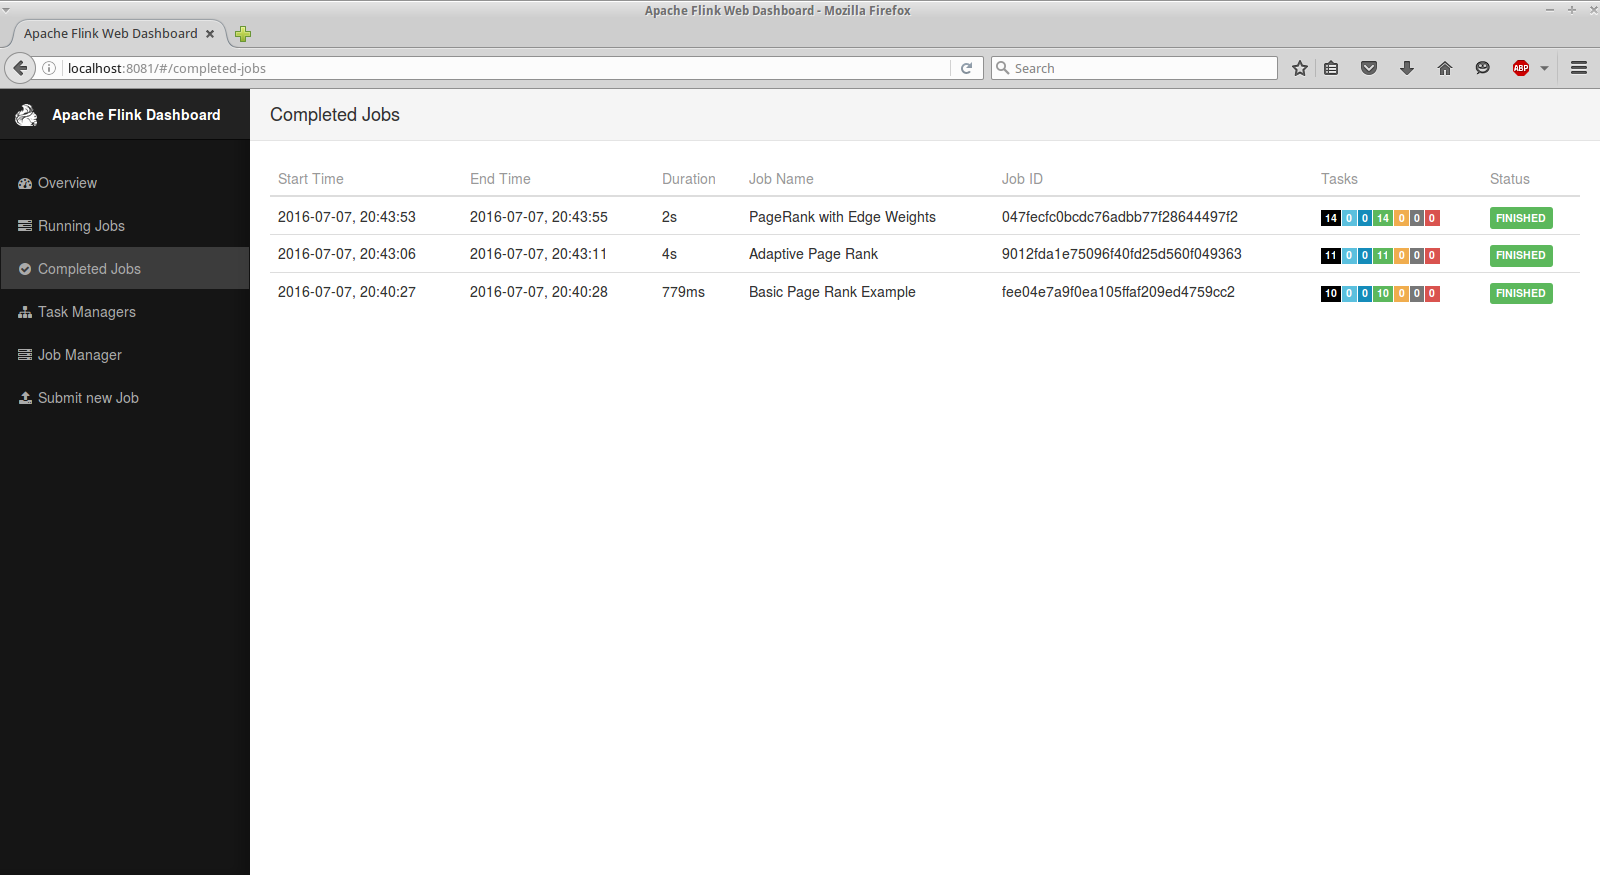
\includegraphics[width=\textwidth]{medium.png}

\end{figure}
\end{frame}
% ------------------------------------------------------------------------------

% ------------------------------------------------------------------------------
\begin{frame}
\frametitle{Results: experiment 1}
\begin{figure}

	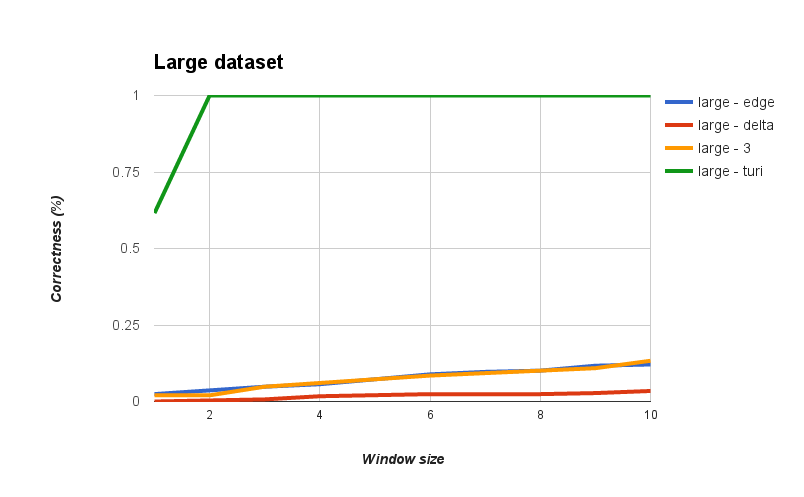
\includegraphics[width=\textwidth]{large.png}

\end{figure}
\end{frame}
% ------------------------------------------------------------------------------

% ------------------------------------------------------------------------------
\begin{frame}
\LARGE These results are ...?
\end{frame}
% ------------------------------------------------------------------------------

% ------------------------------------------------------------------------------
\begin{frame}
\frametitle{Why are the results so bad?}
\LARGE ... Bad
\end{frame}
% ------------------------------------------------------------------------------
% ------------------------------------------------------------------------------
\begin{frame}
\frametitle{Why are the results so bad?}
\LARGE Any ideas?
\end{frame}
% ------------------------------------------------------------------------------

% ------------------------------------------------------------------------------
\begin{frame}
\frametitle{Why are the results so bad?}
\begin{figure}

	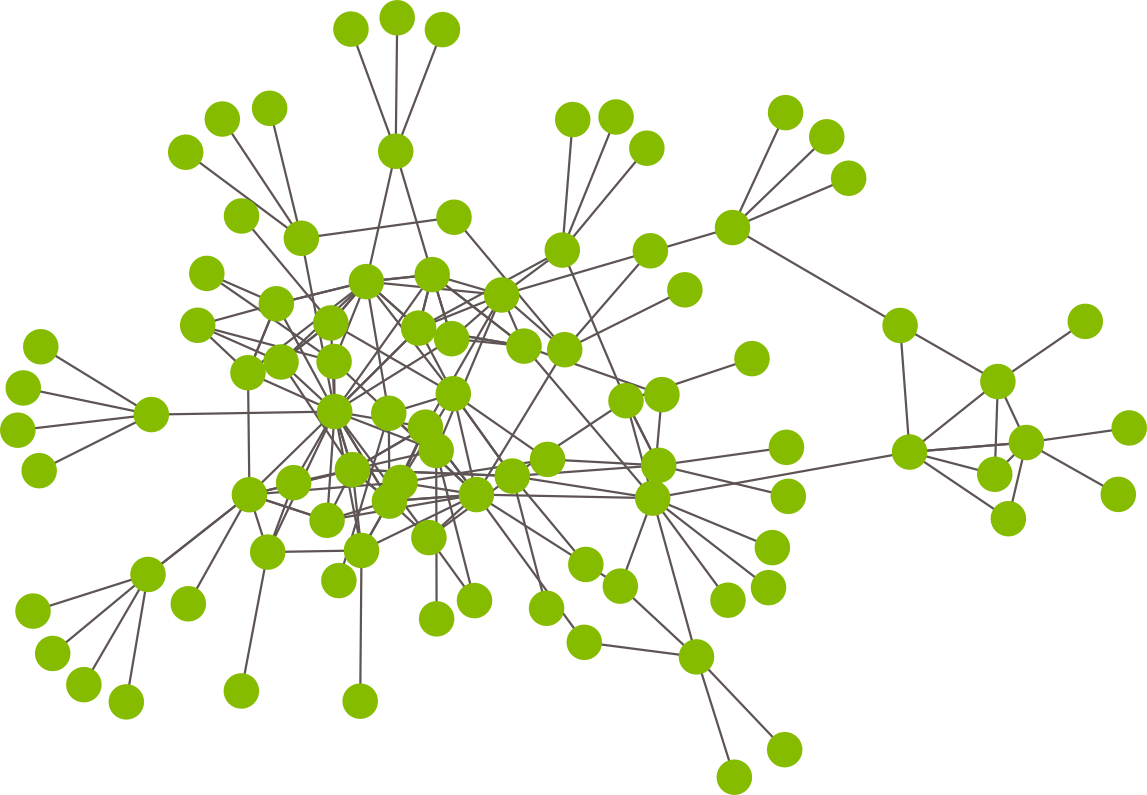
\includegraphics[width=\textwidth]{smallgraph.png}

\end{figure}
\end{frame}
% ------------------------------------------------------------------------------

% ------------------------------------------------------------------------------
\begin{frame}
\frametitle{Why are the results so bad?}
\begin{figure}

	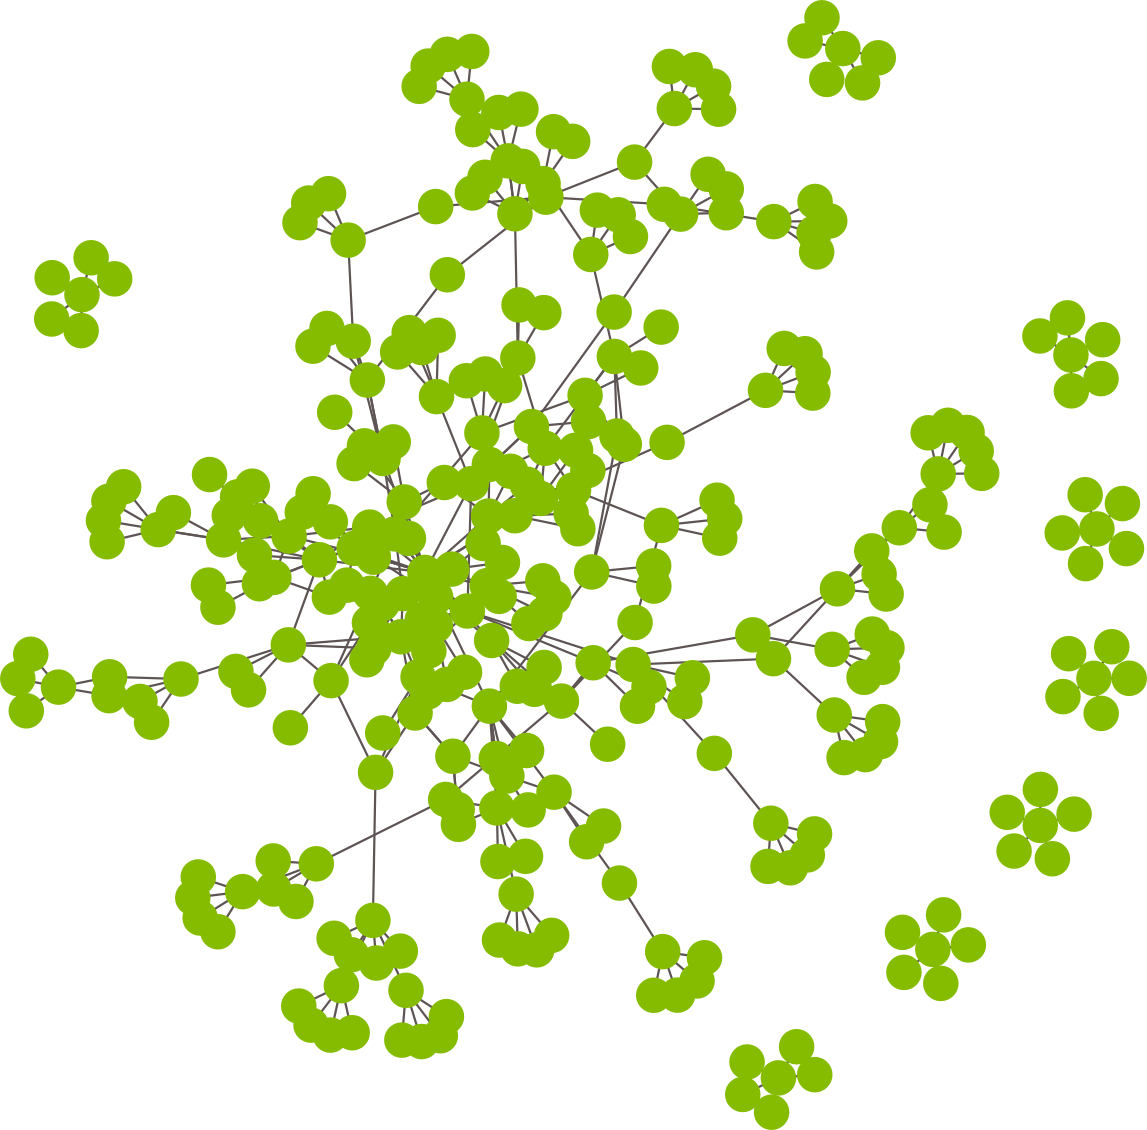
\includegraphics[width=0.7\textwidth]{mediumgraph.png}

\end{figure}
\end{frame}
% ------------------------------------------------------------------------------

% ------------------------------------------------------------------------------
\begin{frame}
\frametitle{Why are the results so bad?}
\begin{figure}

	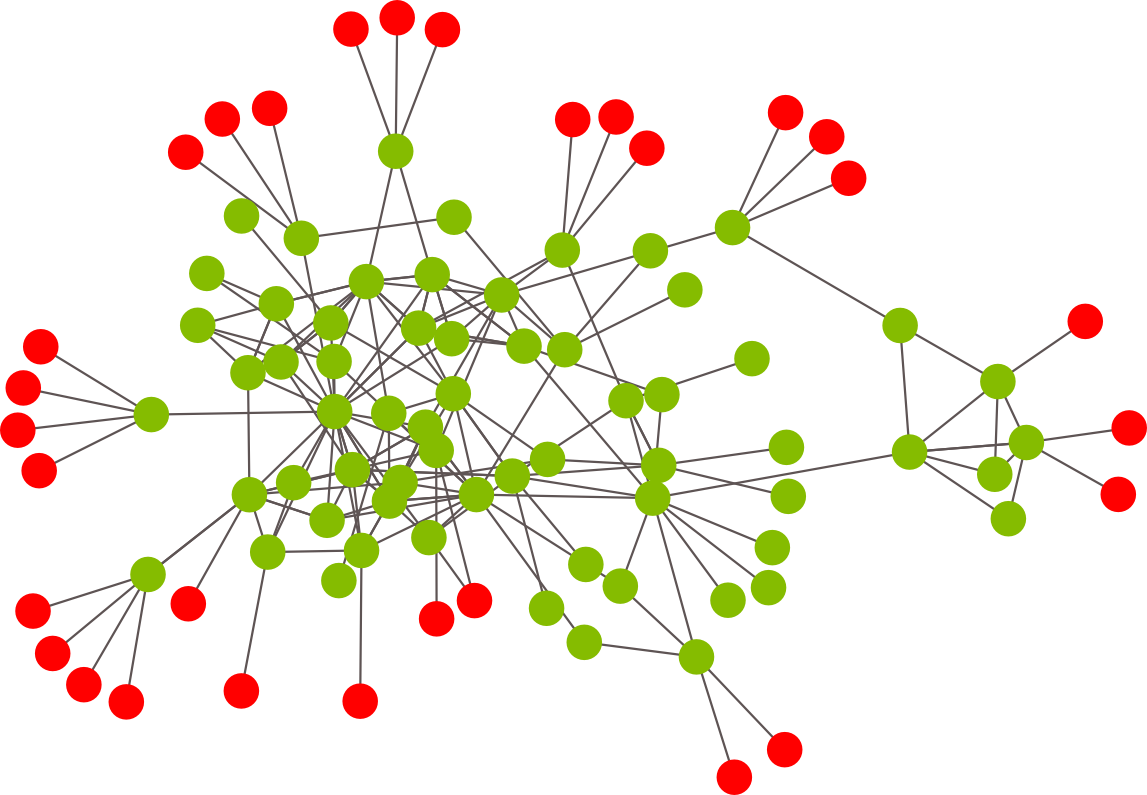
\includegraphics[width=\textwidth]{smallredgraph.png}

\end{figure}
\end{frame}
% ------------------------------------------------------------------------------

% ------------------------------------------------------------------------------
\begin{frame}
\frametitle{Why are the results so bad?}
\begin{figure}

	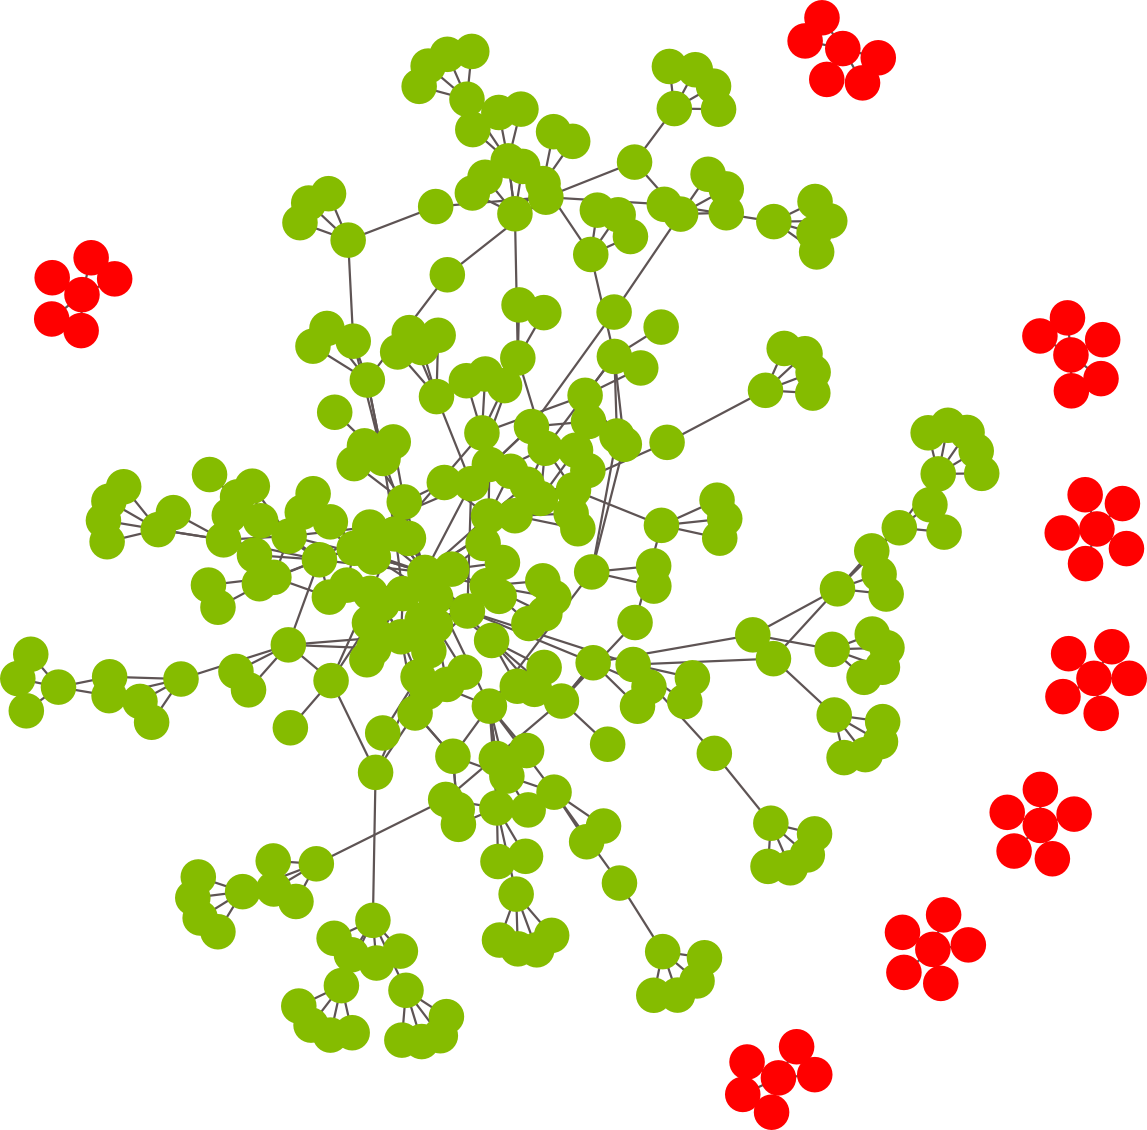
\includegraphics[width=0.7\textwidth]{mediumredgraph.png}

\end{figure}
\end{frame}
% ------------------------------------------------------------------------------


% ------------------------------------------------------------------------------
\begin{frame}
\frametitle{Why are the results so bad?}
\begin{itemize}
\item Implementations expext an incoming and outging edge for every node
\item Dangling nodes
\item Spider traps
\end{itemize}

$\rightarrow$ they are all basic implementations\\
$\rightarrow$ Turi has a advanced implementation
\end{frame}
% ------------------------------------------------------------------------------


% ------------------------------------------------------------------------------
\begin{frame}
\frametitle{Speed of experiment 1}
\begin{figure}

	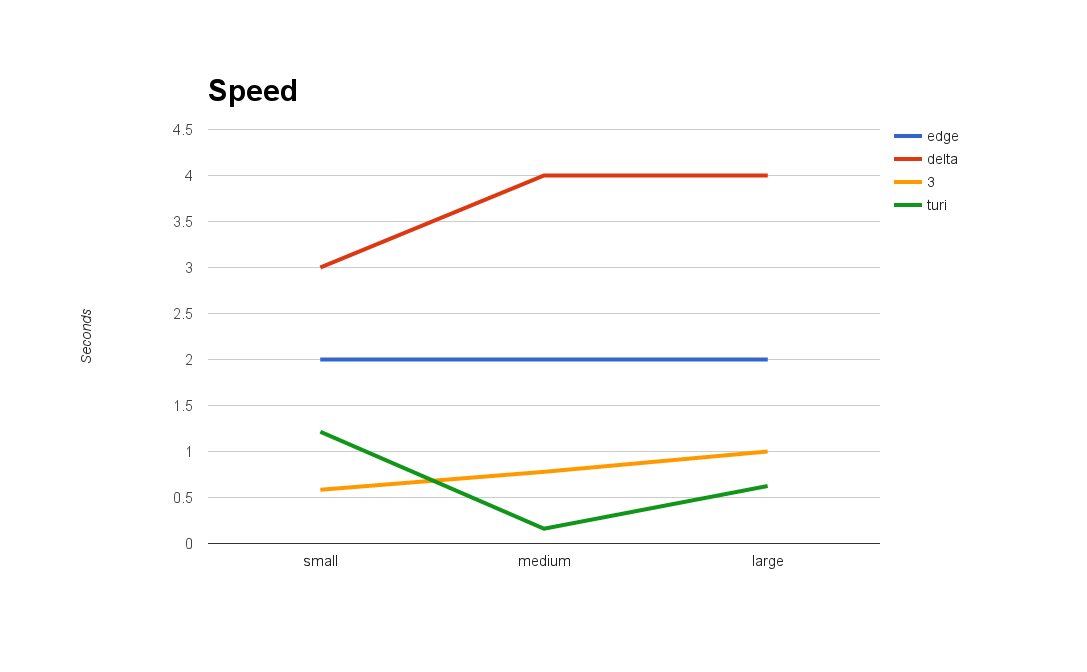
\includegraphics[width=0.9\textwidth]{speeds.png}

\end{figure}
$\rightarrow$ no huge differences with Turi
\end{frame}
% ------------------------------------------------------------------------------

\begin{frame}
\frametitle{Experiment 2}
\begin{figure}

	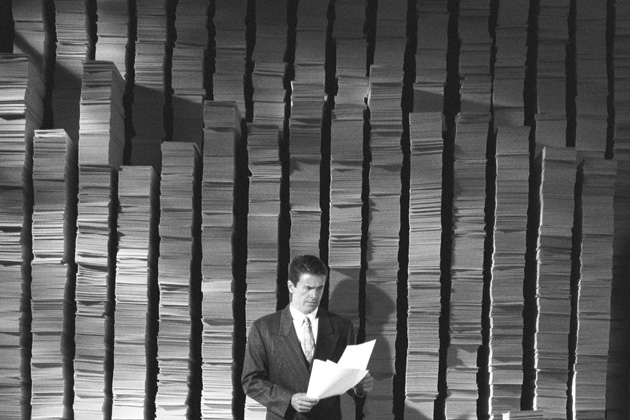
\includegraphics[width=0.9\textwidth]{huge.jpg}

\end{figure}

\end{frame}

% ------------------------------------------------------------------------------
\begin{frame}
\frametitle{Speed of experiment 2}
\begin{table}
\centering
\begin{tabular}{|c|c|c|c|c|}
\hline
Algorithm & Edge & Delta & 3 & Turi\\
\hline
Time (s) & 633 & 549 & 14 & 45\\
\hline
\end{tabular}
\end{table}

\begin{itemize}
\item First two algortihms are a lot slower $\backsim$ 10 times.
\item Algorithm 3 cheats with the filtering
\end{itemize}

\end{frame}
% --

% ------------------------------------------------------------------------------
\begin{frame}

\begin{figure}

	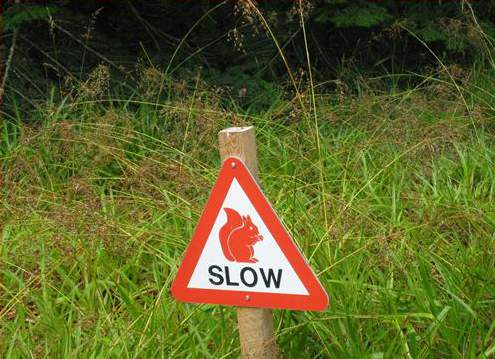
\includegraphics[width=\textwidth]{slow.jpg}

\end{figure}
\end{frame}
% ------------------------------------------------------------------------------


% ------------------------------------------------------------------------------
\begin{frame}
\frametitle{Speed of experiment 2}
\begin{figure}

	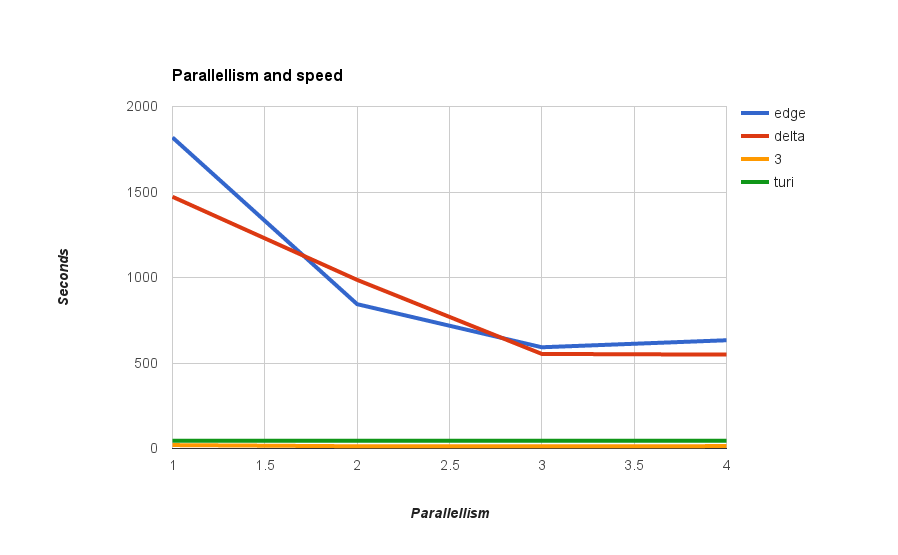
\includegraphics[width=\textwidth]{parallellism.png}

\end{figure}
\end{frame}
% ------------------------------------------------------------------------------

